\documentclass[11pt,a4paper]{article}
\usepackage[T1]{fontenc}
\usepackage[utf8]{inputenc}
\usepackage{lmodern,microtype}
\usepackage{amsmath,amssymb,amsthm,mathtools,bm}
\usepackage{booktabs,array,tabularx,longtable}
\usepackage{graphicx,float,caption}
\usepackage{xcolor}
\usepackage[margin=20mm]{geometry}
\usepackage{enumitem}
\usepackage{fancyhdr}
\usepackage[hidelinks]{hyperref}
\hypersetup{
  pdftitle={FIN ST28--ST45: Carrier-Invariant Information and Symmetry Breaking},
  pdfauthor={Krzysztof Żuchowski},
  pdfsubject={Analytical and computational execution of FIN programs ST28--ST45},
  pdfkeywords={FIN, carrier invariance, operational information, symmetry breaking, positive feedback, spectral operator, selector}
}
\setlength{\parindent}{0pt}
\setlength{\parskip}{0.50em}
\setlength{\emergencystretch}{2em}
\setlength{\headheight}{14pt}
\setlist[itemize]{leftmargin=1.55em,itemsep=0.16em,topsep=0.2em}
\setlist[enumerate]{leftmargin=1.75em,itemsep=0.16em,topsep=0.2em}
\pagestyle{fancy}
\fancyhf{}
\lhead{FIN ST28--ST45}
\rhead{Release 10.57}
\cfoot{\thepage}
\newtheorem{theorem}{Theorem}[section]
\newtheorem{proposition}[theorem]{Proposition}
\newtheorem{corollary}[theorem]{Corollary}
\newcommand{\proven}{\textcolor{green!40!black}{\textbf{[PROVEN]}}}
\newcommand{\strong}{\textcolor{blue!70!black}{\textbf{[STRONG EVIDENCE]}}}
\newcommand{\conditional}{\textcolor{black!60}{\textbf{[CONDITIONAL]}}}
\newcommand{\failed}{\textcolor{red!72!black}{\textbf{[FAILED TEST]}}}
\newcommand{\blocked}{\textcolor{red!72!black}{\textbf{[BLOCKED]}}}
\newcommand{\statusboundary}{\textcolor{orange!80!black}{\textbf{[BOUNDARY]}}}
\newcommand{\resultbox}[1]{\begin{center}\fcolorbox{blue!60!black}{blue!4}{\parbox{0.92\textwidth}{#1}}\end{center}}

\begin{document}

\pagenumbering{gobble}
\begin{titlepage}
\centering
\vspace*{1.30cm}
{\LARGE\bfseries FIN ST28--ST45\par}
\vspace{0.35cm}
{\Large Carrier-Invariant Information and Symmetry Breaking\par}
\vspace{0.40cm}
{\large Interval collision certification, state-dependent algebras, refinement obstructions, finite-count falsification, and operational carrier equivalence\par}
\vspace{1.10cm}
{\Large Krzysztof Żuchowski\par}
\vspace{0.24cm}
{\large Independent Researcher --- Fractal Information Theory Project\par}
{\large ORCID: 0009-0002-0909-3613\par}
\vspace{0.90cm}
{\large FIN Release 10.57 --- Version 1.0.0\par}
{\large August 10, 2026\par}
\vfill
\begin{minipage}{0.89\textwidth}
\textbf{Scope.} This report executes ST28--ST39 recommended by Release 10.56 and adds ST40--ST45 to test two new questions: whether information can be invariant under a change of carrier, and whether symmetry can enable state selection through a separate positive-feedback instability.\par
\textbf{Method.} Finite-dimensional theorems, a frozen-coefficient interval certificate, exact rank calculations, synthetic preregistrations, countermodels, deterministic simulations, and twenty live acceptance tests are included.\par
\textbf{Epistemic rule.} ``Carrier independent'' means invariant under faithful transport of the complete operational experiment. It does not mean that information exists without a realization. Symmetry supplies equivalent alternatives; it is not itself amplification.\par
\textbf{Repository.} \url{https://github.com/hyconiek/Fractal-Nadsoliton-Theory}\par
\textbf{License.} CC BY 4.0.
\end{minipage}
\end{titlepage}
\pagenumbering{arabic}

\begin{abstract}
This report closes eighteen local research programs. ST28 upgrades the ST16 stability transition to a proof-grade unique-root certificate for the explicitly frozen decimal coefficient model:
\[
1.278014751804222\le s_*\le1.2780147518366733.
\]
The interval width is $3.25\times10^{-11}$ and the positive-root derivative is bounded below by $0.530298$. This does not yet interval-regenerate the transcendental strict weights or the upstream memory state.

ST29 proves that a state-dependent density observable can escape the seven-dimensional invariant algebra: a reflection-symmetric localized orbit member generates a $74$-dimensional algebra, while a generic distinct density has scalar joint commutant and generates all of $M_{12}(\mathbb C)$. The symmetric law, however, canonically supplies an orbit and not one orbit member. ST30 proves that ordinary associativity of dyadic refinement is automatic and leaves a new free fine parameter at every scale. ST31 then falsifies the practical strength of the previous ideal mixed-channel test at the declared budget: 2,500 counts per preparation give only $4.75\%$ detection power against the specified alteration. ST32 proves a polynomial long-range influence bound without Markov positivity. ST33 classifies the reflection-compatible cycle fluxes as $0$ and $\pi$, while proving that the phase gradient of any single state has trivial holonomy. ST34 proves existence and set stability of a nonzero minimizer for a constructed saturating DNLS energy, but its best multistart candidate is uniform; no localized soliton evidence is obtained.

ST36 proves the remaining scale-identifiability orbits. ST37 gives a frozen synthetic noise-and-clock-nuisance detection curve. ST38 refutes, within the declared one-vector construction class, the possibility that one strict-sourced state simultaneously provides a canonical selector, the full matrix algebra, and nontrivial holonomy. ST39 reduces the present physical-completion obligations to nine relatively independent axiom groups.

The new carrier study supplies the main conceptual result. ST40 proves exact invariance of every finite record probability under simultaneous transport of generator, state, preparations, and effects; the maximum residual is $8.89\times10^{-16}$. Transporting only the generator while keeping the instruments fixed changes the record by total variation $0.14987$, despite identical spectra. ST41 therefore identifies the minimal candidate invariant as the operational isomorphism class of algebra, states, dynamics, preparations, instruments, composition, and records---not the spectrum alone. ST42 proves the corresponding obstruction: information may be independent of which faithful carrier realizes it, but operational information is undefined after all realization structure is removed.

ST43 separates symmetry from feedback in a constructed $C_{12}$-equivariant polar flow. Symmetry supplies twelve equivalent alternatives; positive linear gain destabilizes the symmetric state, saturation bounds growth, and an equivariant angular term selects an orbit member. ST44 shows that the strict operator itself provides a canonical two-dimensional degenerate subspace but no preferred axis; a selected axis yields only the $74$-dimensional reflection-anchored algebra. ST45 finally proves that unitary and heat channels can share $A$ while remaining dynamically inequivalent on every positive mode. Thus the new hypothesis is mathematically meaningful, but FIN has not shown that distinct physical media instantiate one operational information object, nor that its feedback gain or realized history is generated by the strict core.
\end{abstract}

\textbf{Status vocabulary.} \proven{} denotes an analytic or exact finite result in the declared model. \strong{} denotes robust but non-interval numerical evidence. \conditional{} denotes a result after named inserted premises. \failed{} records a test that did not achieve its declared discrimination goal. \blocked{} marks an unavailable formal replay. \statusboundary{} gives the exact non-implication.

\tableofcontents
\newpage

\section{Research questions and starting object}

The strict finite working object is
\[
W_{xx}=0,\qquad
W_{xy}=\frac{\cos(0.18575d(x,y)+0.16250)}{1+d(x,y)^{1.8}}\quad(x\ne y),
\qquad A=sI-W\succeq0,
\]
where $s$ is the off-diagonal row sum. The explicit zero diagonal is essential: inserting the scalar kernel at $d=0$ would define a different matrix and would be inconsistent with the quoted row sum.

The programs address two distinct layers:
\begin{align*}
\text{existing continuation: }&\quad \text{certification, selector, refinement, locality, nonlinear and scale tests},\\
\text{new conceptual continuation: }&\quad \text{carrier invariance and symmetry-enabled selection}.
\end{align*}
The second layer is not an assumption that FIN is a Theory of Everything. It asks whether the proposed ideas can be stated as falsifiable finite mathematics.

\resultbox{\textbf{Answer in one sentence.} Information can be fundamentally independent of a \emph{particular} carrier when different realizations are isomorphic as complete operational processes; it cannot be operationally independent of \emph{every} realization, and current FIN has not proved that actual physical media realize the required isomorphism.}

\section{Outcome matrix}

\small
\begin{longtable}{@{}p{0.055\textwidth}p{0.32\textwidth}p{0.21\textwidth}p{0.34\textwidth}@{}}
\toprule
ID & Object & Outcome & Exact boundary\\
\midrule
\endfirsthead
\toprule
ID & Object & Outcome & Exact boundary\\
\midrule
\endhead
ST28 & Frozen-coefficient Jordan certificate & \proven{} & Upstream transcendental coefficients not interval-regenerated\\
ST29 & State-orbit algebra & \proven{} & Generic state is constructed, not strict-sourced\\
ST30 & Dyadic coherence & \proven{} no-selection & Stronger scale law remains possible\\
ST31 & Finite-count common-generator test & \failed{} & Synthetic receiver; only $4.75\%$ power\\
ST32 & Long-range influence & \proven{} & Polynomial tail, not a causal cone\\
ST33 & Cycle holonomy & \proven{} & $\pi$ sector is not selected\\
ST34 & Saturating DNLS minimizer & \proven{} $+$ \strong{} & Candidate uniform; no soliton evidence\\
ST35 & Lean replay & \blocked{} & No cached toolchain\\
ST36 & Sector-scale identification & \proven{} & Does not supply SI units\\
ST37 & Nuisance-robust adversary & \strong{} & Synthetic noise model\\
ST38 & Joint state closure & \proven{} no-go & Multi-component/projective objects remain open\\
ST39 & Relative axiom graph & \proven{} & Minimal only for declared targets/classes\\
ST40 & Carrier-neutral operation & \proven{} & Complete transport is required\\
ST41 & Information hierarchy & \proven{} & Completeness is relative to finite experiments\\
ST42 & Realization-removal obstruction & \proven{} & Operational, not metaphysical, theorem\\
ST43 & Symmetry/feedback polar flow & \conditional{} $+$ \strong{} & Gain and anisotropy inserted\\
ST44 & Strict degenerate-mode selector & \proven{} partial & No preferred axis or gain source\\
ST45 & Medium versus channel equivalence & \proven{} & No physical carrier identification\\
\bottomrule
\end{longtable}
\normalsize

\section{ST28 --- Certified stability-collision root}

ST16 reduced the hidden Hamiltonian-memory collision to
\[
p(x)=(c_2+c_3)x^2+2c_1x+c_0=0,\qquad x=s^{-1}.
\]
ST28 surrounds the frozen binary64 stationary state by an $\ell^\infty$ box of radius $10^{-13}$, propagates that box through the coefficient forms, and pays a $2\times10^{-14}$ rounding allowance. The accepted coefficient intervals are
\begin{align*}
0.2671565201183534&\le c_2+c_3\le0.2671565201188946,\\
0.11221794518323411&\le2c_1\le0.11221794518634101,\\
-0.2513728361132897&\le c_0\le-0.25137283610551603.
\end{align*}
The inverse Newton image is strictly contained in every tested box from $10^{-13}$ through $10^{-9}$. Monotonicity on the positive root interval then gives:

\begin{theorem}[Frozen-coefficient collision certificate]
For the declared exact-decimal coefficient model, one and only one positive collision speed lies in
\[
1.278014751804222\le s_*\le1.2780147518366733.
\]
The derivative of $p$ is at least $0.5302984403$ throughout the isolating interval.
\end{theorem}

\begin{figure}[H]
\centering
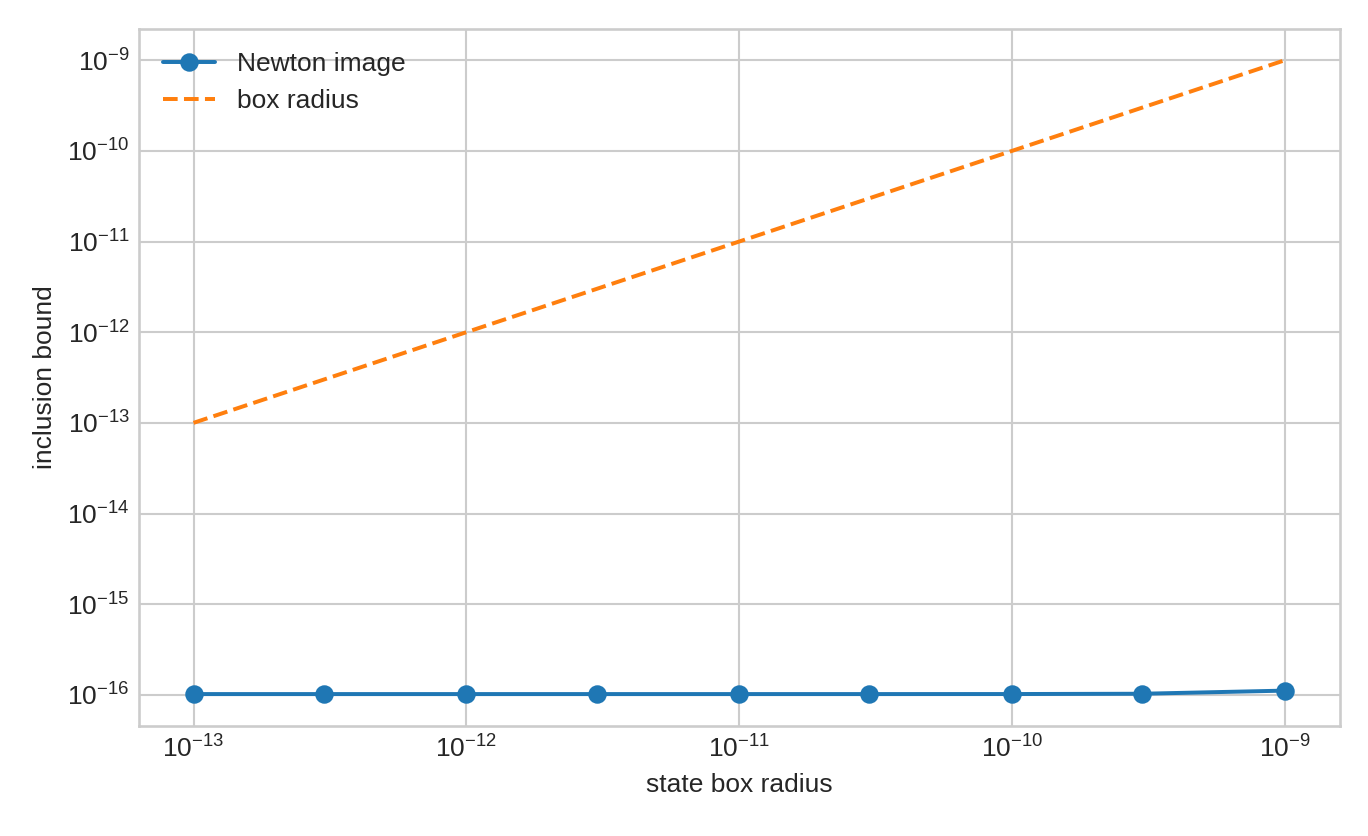
\includegraphics[width=0.80\textwidth]{FIN_ST28_ST45_Figures/st28_interval_jordan_certificate.png}
\caption{Strict inclusion of the interval Newton image. This certifies the frozen decimal coefficient model, not the complete upstream construction.}
\end{figure}

\statusboundary{} This is a genuine theorem about the frozen coefficients, not yet about coefficients rederived by interval evaluation of every strict transcendental weight and memory solve. ST46 is designed to close precisely that gap.

\section{ST29 and ST38 --- State-dependent selector and algebra tests}

Let $D_\psi=\operatorname{diag}(|\psi_0|^2,\ldots,|\psi_{11}|^2)$. The algebra generated by $A$ and $D_\psi$ is computed through the finite bicommutant theorem rather than unstable word iteration.

\begin{proposition}[Generic state algebra completion]
If $D_\psi$ has distinct diagonal entries and the support graph of $A$ is connected, then every matrix commuting with both $A$ and $D_\psi$ is scalar. Consequently,
\[
C^*(A,D_\psi)=M_{12}(\mathbb C).
\]
\end{proposition}

The three audited cases are:
\begin{center}
\begin{tabular}{@{}lrrr@{}}
\toprule
State density & Orbit size & Joint commutant & Algebra dimension\\
\midrule
Uniform & 1 & 22 & 7\\
Localized, reflection symmetric & 12 & 2 & 74\\
Generic & 24 & 1 & 144\\
\bottomrule
\end{tabular}
\end{center}
The group average of the generic orbit returns the uniform density to residual $6.21\times10^{-17}$. Thus a symmetric rule can canonically generate the orbit, but cannot canonically choose one member.

ST38 combines density selection, algebra generation, pair current, and phase-gradient holonomy. A generic complex state has algebra dimension $144$ and total absolute pair current $0.96787$, but its phase-gradient holonomy differs from one by only $5.47\times10^{-16}$. Every one-state link $g_{x,x+1}=e^{i(\theta_{x+1}-\theta_x)}$ telescopes:
\[
\prod_{x=0}^{11}g_{x,x+1}=1.
\]

\begin{theorem}[One-vector joint-closure obstruction]
Within the declared construction class, one strict-sourced vector cannot simultaneously provide (i) a canonical orbit member, (ii) the full matrix algebra, and (iii) nontrivial cycle holonomy. A generic vector can supply (ii) and current, but not a canonical origin or nontrivial holonomy.
\end{theorem}

\begin{figure}[H]
\centering
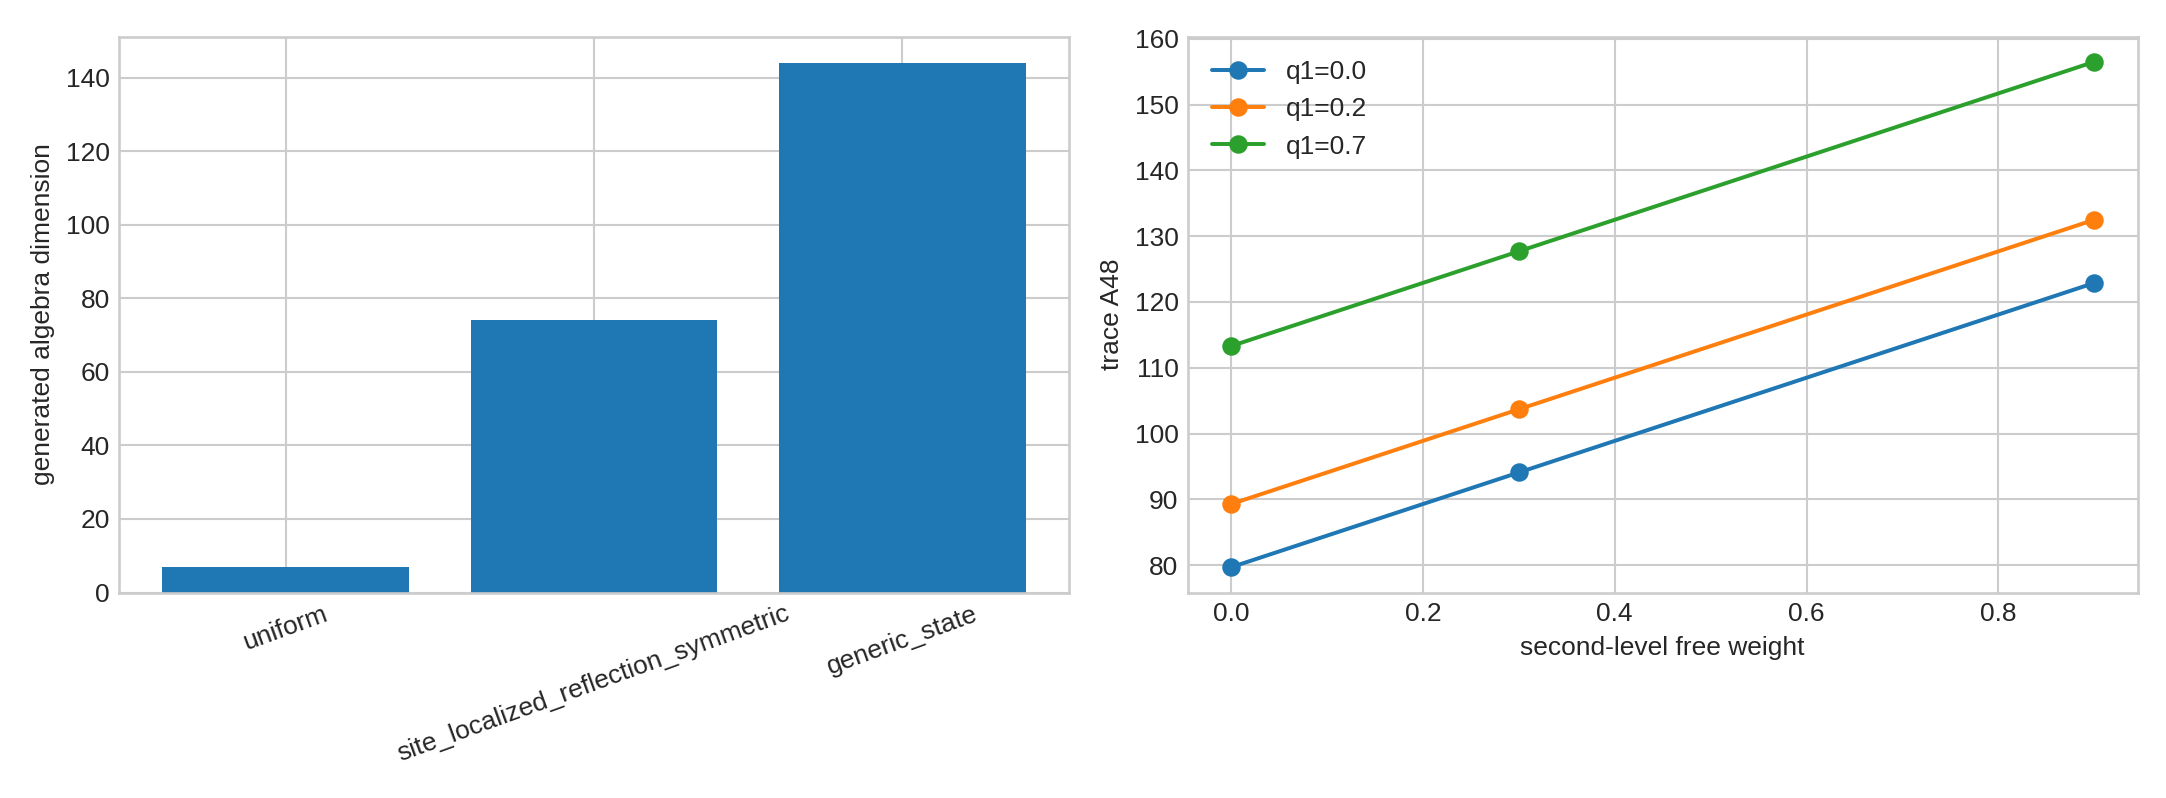
\includegraphics[width=0.96\textwidth]{FIN_ST28_ST45_Figures/st29_state_algebra_st30_coherence.png}
\caption{Left: a state can enlarge the invariant algebra, but greater algebraic separation accompanies a larger unresolved symmetry orbit. Right: coherent dyadic refinements remain nonunique.}
\end{figure}

\statusboundary{} State dependence is a valid route out of the ST17 invariant-algebra no-go. It does not discharge QW-2191 because the current strict core supplies neither the generic state nor the realized orbit member.

\section{ST30 --- Associativity does not select a refinement}

Let $J_n:\mathbb C^n\to\mathbb C^{2n}$ repeat coarse data periodically. The ST18 lift satisfies
\[
A_{2n}(q_n)J_n=J_nA_n
\]
for every nonnegative new fine antipodal weight $q_n$. Therefore
\[
A_{4n}(q_{2n})J_{2n}J_n=J_{2n}J_nA_n
\]
holds by composition for every pair $(q_n,q_{2n})$.

Nine tested pairs have maximum intertwining residual $2.40\times10^{-15}$, yet the corresponding $A_{48}$ matrices differ by as much as $13.1727$ in Frobenius norm.

\begin{theorem}[Plain coherence nonselection]
Associativity of the existing intertwining squares is automatic and imposes no relation between the newly introduced fine weights. At least one free nonnegative parameter survives per dyadic level.
\end{theorem}

This refutes the hope that diagrammatic path independence alone selects the continuum tower. A stronger condition must couple scales, for example a scale-stationary local rule, a universal action, or a compression law with a proved fixed point.

\section{ST31 and ST37 --- Finite-count and nuisance falsification}

\subsection{ST31: the ideal common-generator test loses power}

For vertex preparations and vertex outcomes the mixed channel is normalized into
\[
p_{y|x}(A_H,A_U)=
\frac{|[e^{-itA_U}e^{-\tau A_H}]_{yx}|^2}
{\sum_z|[e^{-itA_U}e^{-\tau A_H}]_{zx}|^2}.
\]
The frozen protocol uses $t=0.47$, $\tau=0.61$, 2,500 counts for each of twelve preparations, twelve outcomes, and a Pearson threshold $172.7108$ at nominal level $0.01$ with 132 degrees of freedom. The alternative is
\[
A_U=A+0.06\,vv^T,\qquad v\perp\bm1.
\]
Across 400 common and 400 altered trials:
\[
\widehat{\alpha}=0.0125,\qquad \widehat{\text{power}}=0.0475.
\]

\failed{} The receiver has essentially no useful power for the declared alternative at this budget. This is not evidence for the common-generator hypothesis. It demonstrates that an exact operator identity can become practically uninformative after a specific measurement map and finite sampling.

\begin{figure}[H]
\centering
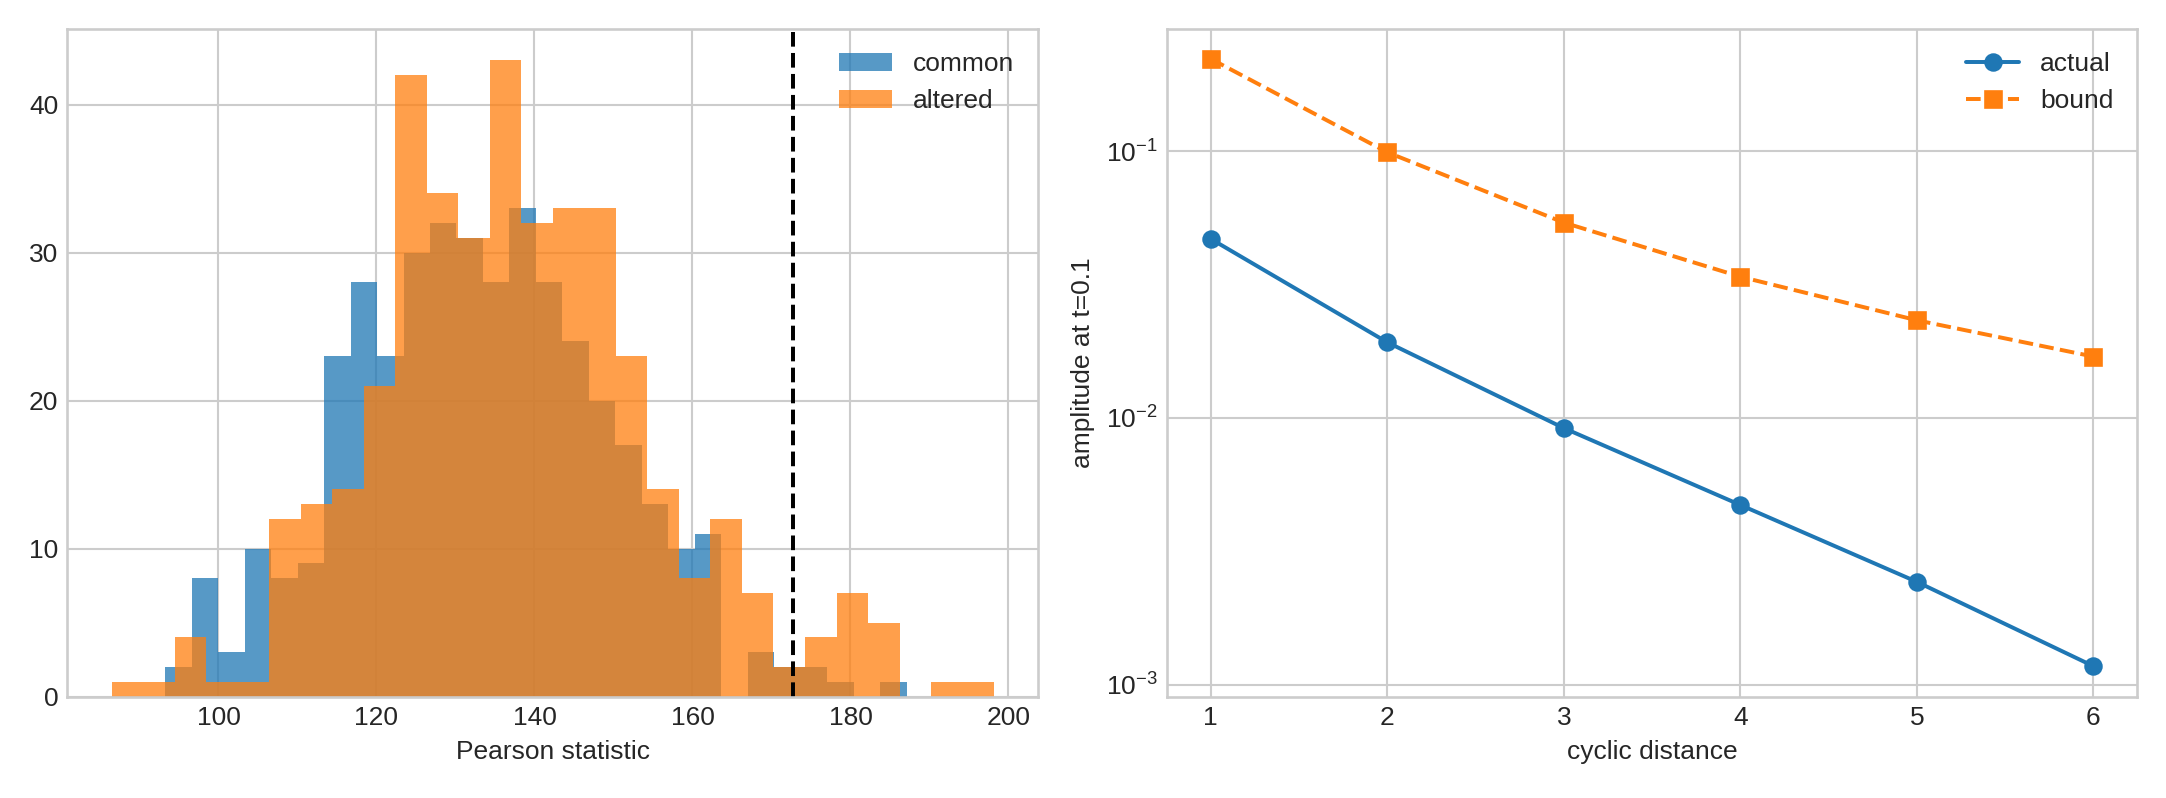
\includegraphics[width=0.96\textwidth]{FIN_ST28_ST45_Figures/st31_counts_st32_polynomial_bound.png}
\caption{Left: the finite-count null and altered statistic distributions strongly overlap. Right: the analytic long-range envelope safely bounds the sampled strict amplitudes but is deliberately loose.}
\end{figure}

\subsection{ST37: matrix-level adversaries under nuisance}

ST37 freezes a different synthetic protocol before holdout: complex entry noise $\sigma=5\times10^{-4}$, clock nuisance $\pm0.5\%$, a 21-point time grid, and a 99th-percentile threshold learned from 400 null samples. Isospectral adversaries $QAQ^T$ fix the uniform mode while rotating the positive subspace.

\begin{center}
\begin{tabular}{@{}rrr@{}}
\toprule
Rotation size & Median score & Detection power\\
\midrule
0.003 & 0.001851 & 0.240\\
0.010 & 0.002829 & 1.000\\
0.030 & 0.006851 & 1.000\\
\bottomrule
\end{tabular}
\end{center}
The frozen threshold is $0.0019163$ and the independent null false-rejection rate is $0.0025$.

\strong{} These numbers establish the behavior of the frozen synthetic receiver only. They are not laboratory sensitivity, because neither the Gaussian entry-noise law nor the clock interval has been calibrated to apparatus.

\begin{figure}[H]
\centering
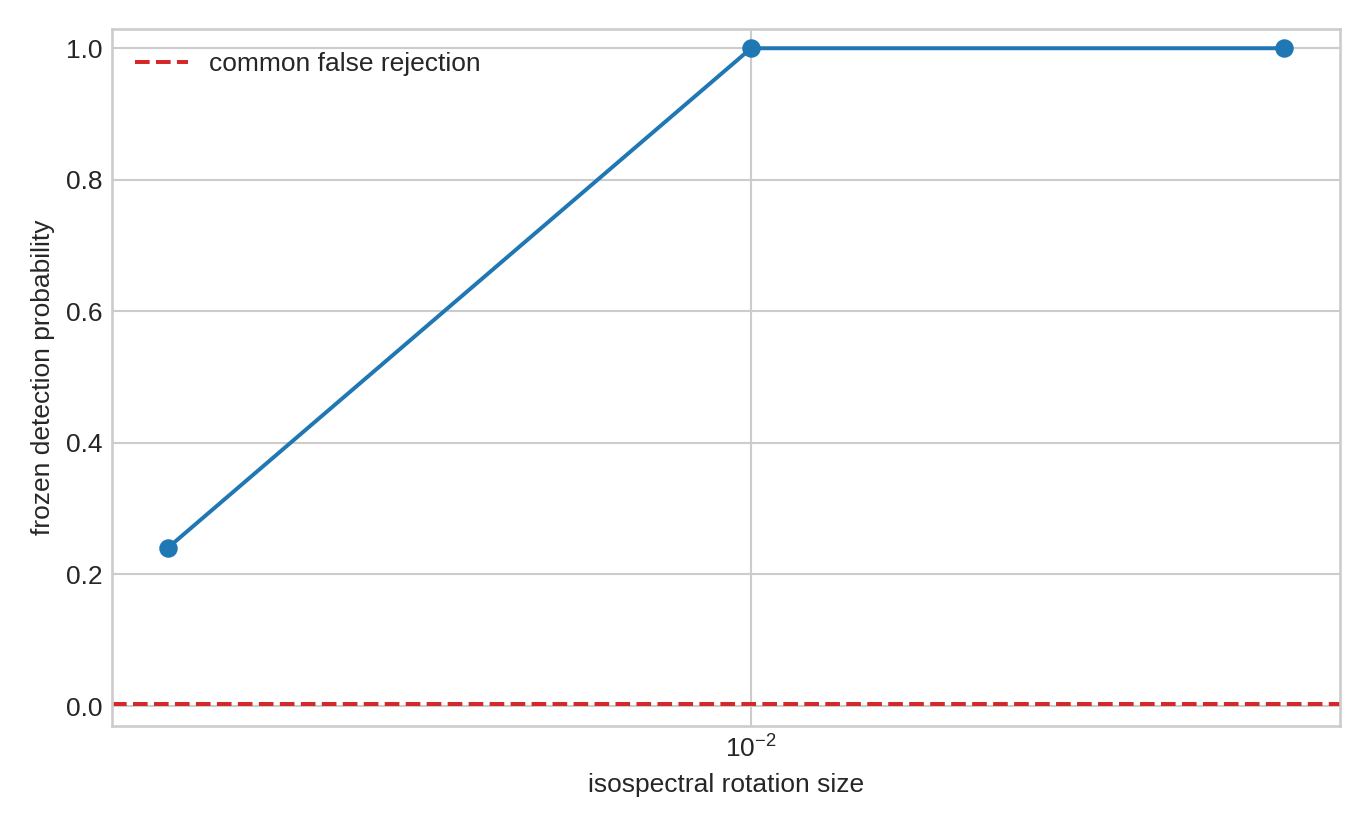
\includegraphics[width=0.72\textwidth]{FIN_ST28_ST45_Figures/st37_nuisance_detection.png}
\caption{Frozen synthetic detection curve for isospectral positive-subspace rotations.}
\end{figure}

\section{ST32 --- A polynomial influence theorem without Markovity}

Set $F(r)=(1+r^\eta)^{-1}$ with $\eta>1$. Splitting a convolution sum according to whether $|z|\ge r/2$ or $|r-z|\ge r/2$ yields
\[
(F*F)(r)\le C_FF(r),\qquad
C_F\le2^{\eta+1}\sum_{z\in\mathbb Z}F(|z|).
\]
Consequently, if $|W_{xy}|\le F(d(x,y))$, induction gives
\[
|(W^n)_{xy}|\le C_F^{n-1}F(d(x,y)),
\]
and hence
\[
|[e^{itW}]_{xy}|\le F(d(x,y))\frac{e^{C_F|t|}-1}{C_F}.
\]
For $\eta=1.8$, the certified summability upper bound is $3.57553$ and $C_F\le24.90144$. A finite convolution scan gives only a lower estimate $7.12808$ for the best constant.

\proven{} The result bounds propagation for the signed long-range operator without pretending that $W/s$ is a stochastic kernel. \statusboundary{} The tail is polynomial and nonzero at every distance; it is neither a Lieb--Robinson exponential cone nor Lorentz causality.

\section{ST33 --- Reflection, discrete flux, and the one-state no-go}

Gauge classes of $U(1)$ connections on a cycle are classified by total flux $\Phi\bmod2\pi$. Reflection reverses orientation and sends $\Phi\mapsto-\Phi$. Its fixed classes therefore satisfy
\[
2\Phi=0\pmod{2\pi},\qquad \Phi\in\{0,\pi\}.
\]
This leaves a discrete $\pi$ possibility outside the continuous no-go of ST23. But an ordinary single-valued state phase produces only an exact one-form and trivial holonomy. Even a phase winding once around the cycle gives total group holonomy one.

\proven{} The $\pi$ sector is mathematically allowed by reflection. \statusboundary{} It requires an independent link, projective sign, spin structure, or equivalent new object; strict $A$ does not select it.

\section{ST34 --- What the saturating nonlinear model actually produces}

The constructed ST24 $a=0$ potential uses
\[
q(\rho)=\frac{\rho}{1+\rho/R},\qquad
V(\rho)=-\frac12q(\rho)^2+\frac\mu2\rho,
\]
and
\[
E(u)=\frac12u^TAu+\sum_xV(u_x^2),\qquad \mu=0.15, R=2.
\]
Since $q$ saturates and $\mu>0$, $E$ is coercive on the finite state space. Continuity gives a global minimizer; an explicit negative-energy trial proves that the minimizing set is nonzero. The Hamiltonian flow conserves $E$, so the compact set of global minimizers is Lyapunov stable as a set.

Sixty BFGS starts found a best stationary candidate with energy $-8.219889$, gradient residual $1.44\times10^{-10}$, inverse participation ratio $1/12$, and density-uniformity residual $2.78\times10^{-11}$. No stationary candidate crossed the declared localization threshold.

\begin{figure}[H]
\centering
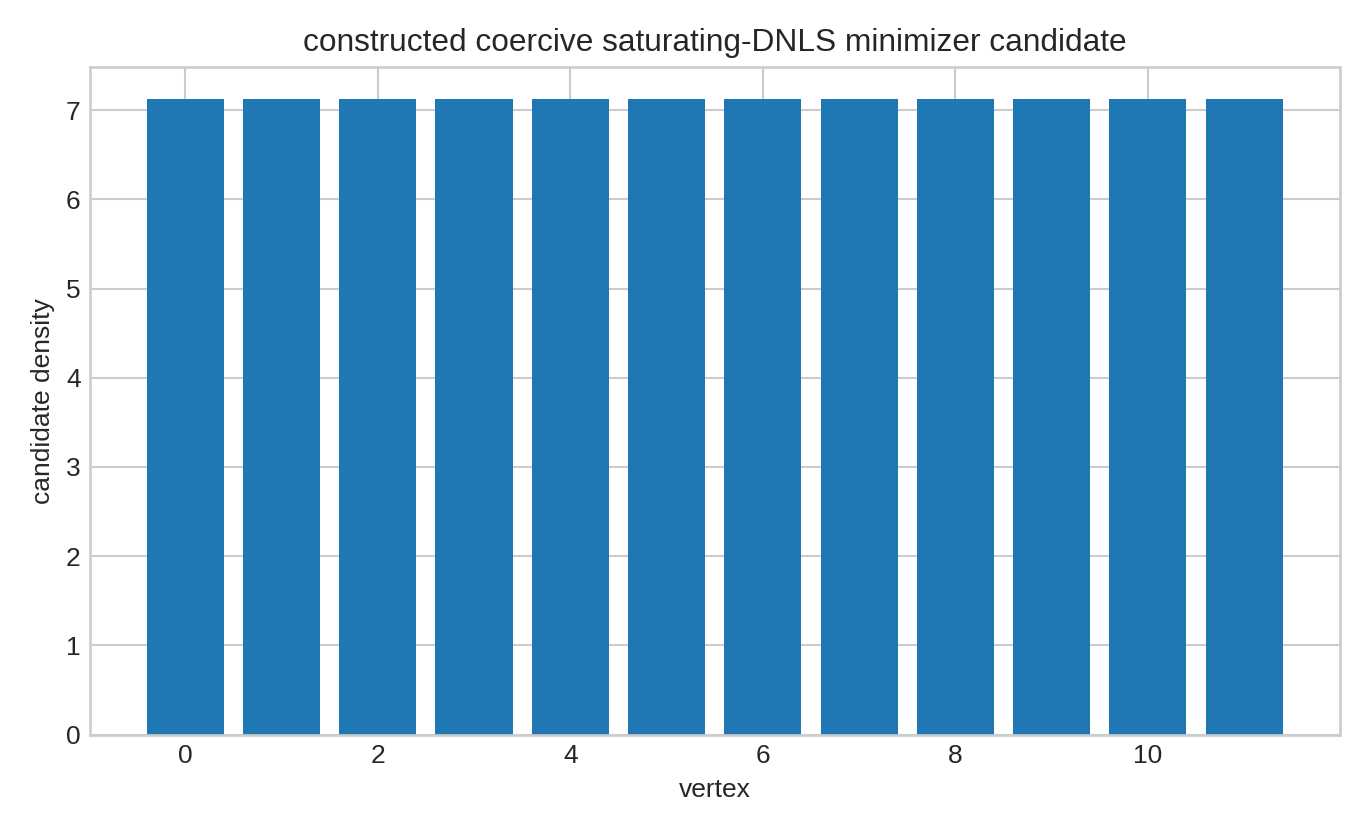
\includegraphics[width=0.75\textwidth]{FIN_ST28_ST45_Figures/st34_saturating_minimizer.png}
\caption{The best constructed nonlinear minimizer candidate is uniform. The nonlinear completion stabilizes a nonzero phase, not a localized soliton in this search.}
\end{figure}

\resultbox{\textbf{Falsification result.} This study does not derive a particle-like object. It proves a nonzero minimizer set for an inserted nonlinear law and finds evidence for a uniform ordered phase. Calling this candidate a soliton would contradict the calculation.}

\section{ST35 and ST36 --- Formal replay and dimensional identifiability}

\subsection{ST35}
The host contains \texttt{lean} and \texttt{elan} launchers but no configured toolchain. No network installation was attempted. Therefore the ST25 source is still not machine checked. A version string without a cached compiler and the required library archive would not constitute replay.

\subsection{ST36}
Channel-specific observables depend on different products:
\[
\omega_U\sim\alpha_U\lambda,qquad
\gamma_H\sim\alpha_H\lambda,qquad
\omega_C\sim\sqrt{\alpha_C\lambda},
\]
with separate affine Green parameters and the Gibbs product $\beta E_*$. Exact symbolic design-matrix ranks give:
\begin{center}
\begin{tabular}{@{}lrrr@{}}
\toprule
Clock assumption & Parameters & Rank & Nullity\\
\midrule
Calibrated channel times & 7 & 6 & 1\\
Uncalibrated channel times & 10 & 6 & 4\\
\bottomrule
\end{tabular}
\end{center}
The calibrated case leaves the Gibbs orbit $(\beta,E_*)\mapsto(c\beta,E_*/c)$. Without clocks, three additional scale--time orbits survive. Thus soliton or mode frequency gives dimensionless phase time and ratios, not seconds. For $e^{-itA}$ the rescaling is $(A,t)\mapsto(cA,t/c)$; for $\cos(t\sqrt A)$ it is $(A,t)\mapsto(cA,t/\sqrt c)$. One fixed physical dimension for $A$ cannot serve both roles without explicit sector maps.

\section{ST39 --- Relative minimal axiom graph}

The accumulated countermodels separate nine current obligation groups:
\begin{enumerate}
\item $A_0$: the strict finite operator;
\item $A_1$: a state-selection event or equivalent orbit-member source;
\item $A_2$: a refinement law;
\item $A_3$: dimensional calibration;
\item $A_4$: preparations, instruments, composition, and records;
\item $A_5$: external custody and empirical data;
\item $A_6$: a nonlinear response law;
\item $A_7$: a connection or projective sector;
\item $A_8$: a temporal realization of the static memory operator.
\end{enumerate}
Removing each group has an explicit witness: ST29 for $A_1$, ST30 for $A_2$, ST36 for $A_3$, ST31/ST37 for $A_5$, ST34 for $A_6$, ST33/ST38 for $A_7$, and ST16/ST28 for $A_8$.

\proven{} This is a relative independence ledger for the declared target family and known construction classes. It is not an absolute theorem that no future object can jointly supply several groups.

\section{ST40--ST42 --- What carrier-independent information can mean}

\subsection{Operational transport}

Let a finite operational realization be
\[
\mathcal R=(\mathcal A,\{\rho_a\},\{\Phi_t\},\{E_b\},\circ,\mathsf{Rec}),
\]
where $\rho_a$ are preparations, $\Phi_t$ are channels, $E_b$ are effects, $\circ$ records composition, and $\mathsf{Rec}$ is the record map. A faithful change of representation by a unitary or orthogonal $Q$ transports every component:
\[
A'=QAQ^*,\quad \rho'_a=Q\rho_aQ^*,\quad E'_b=QE_bQ^*,\quad
\Phi'_t=\operatorname{Ad}_Q\circ\Phi_t\circ\operatorname{Ad}_{Q^*}.
\]
Then
\[
\operatorname{tr}\!\left(E'_b\Phi'_t(\rho'_a)\right)
=\operatorname{tr}\!\left(E_b\Phi_t(\rho_a)\right).
\]

\begin{theorem}[Carrier-neutral operational equivalence]
Every finite record probability is invariant under simultaneous faithful transport of the complete operational realization. Therefore the operational isomorphism class $[\mathcal R]$, rather than a chosen matrix representation, is carrier neutral.
\end{theorem}

The live $12$-state calculation has record residual $8.89\times10^{-16}$. By contrast, replacing $A$ by the isospectral $QAQ^T$ while leaving the vertex state and vertex effects fixed produces total-variation discrepancy $0.1498688$.

\begin{figure}[H]
\centering
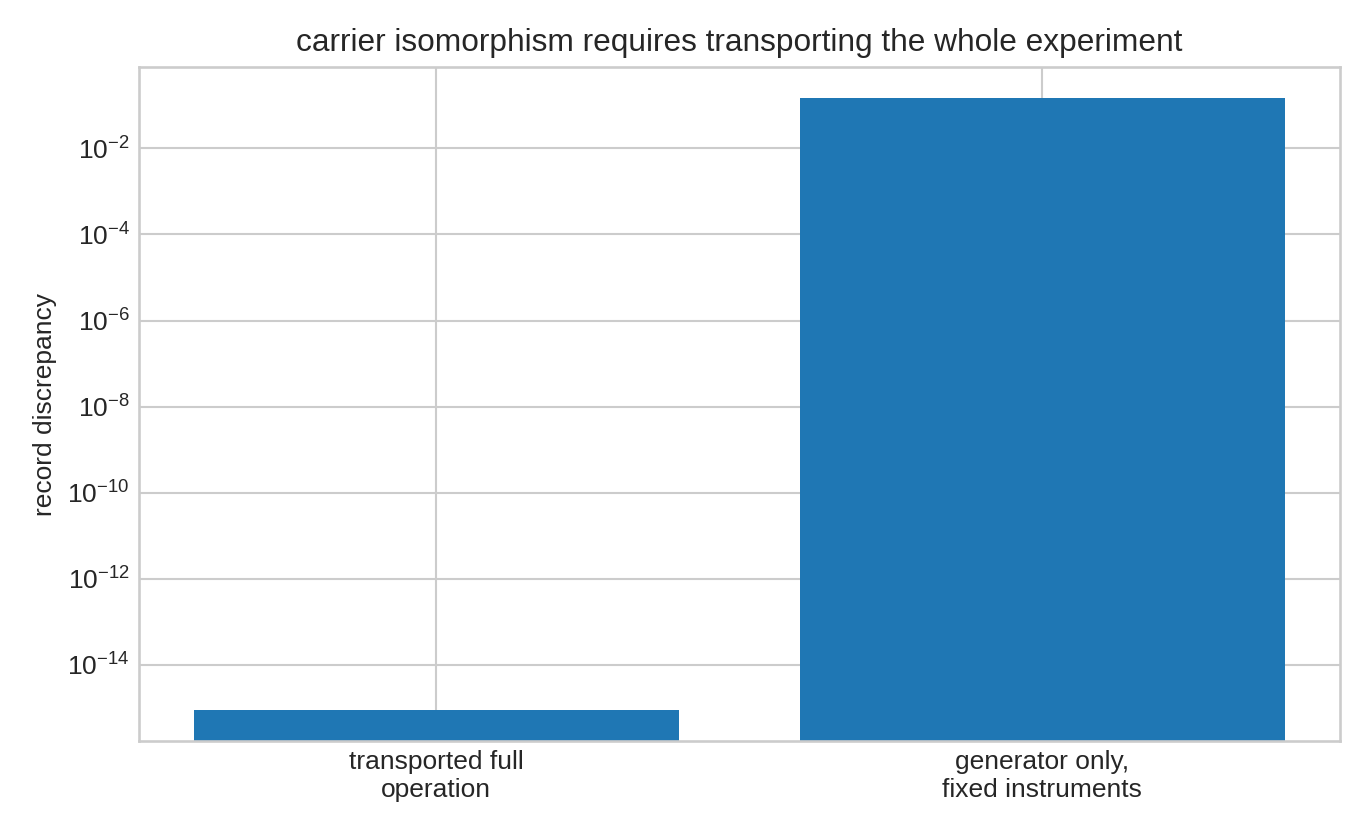
\includegraphics[width=0.75\textwidth]{FIN_ST28_ST45_Figures/st40_carrier_invariance.png}
\caption{Changing coordinates preserves information only when the whole operational experiment is transported. Spectrum-preserving generator replacement with fixed instruments is empirically distinguishable.}
\end{figure}

\subsection{Why the spectrum is too small}

The resulting hierarchy is:
\begin{center}
\begin{tabularx}{0.96\textwidth}{@{}lXl@{}}
\toprule
Level & Data & Complete for the declared finite task?\\
\midrule
$I_0$ & Dimension, entropy-like scalars & No\\
$I_1$ & Eigenvalue multiset & No\\
$I_2$ & Generator and projectors up to simultaneous isomorphism & No\\
$I_3$ & States, channels, instruments, and all record probabilities & Yes\\
$I_4$ & $I_3$ plus composition, calibration, and external provenance & Yes; physically richer\\
\bottomrule
\end{tabularx}
\end{center}
Thus the minimal FIN candidate for ``the same information across carriers'' is
\[
\boxed{[\mathcal A,\text{states},\text{dynamics},\text{preparations},
\text{instruments},\text{composition},\text{records}]_{\cong_{\rm op}}.}
\]
Eigenvalues alone fail because they do not identify how states and instruments sit relative to the eigenspaces.

\subsection{The realization-removal obstruction}

Sequential removal exposes the minimum operational content:
\begin{itemize}
\item without distinguishable states there are no alternatives to encode;
\item without effects and probabilities Shannon or relative information is undefined;
\item without encoding/decoding maps cross-carrier identity is untestable;
\item without record equivalence there is no criterion that the same message survived;
\item without a bath and scale, information does not become thermodynamic entropy or work.
\end{itemize}

\begin{theorem}[No realization-free operational information]
Operational information may be invariant under replacement of one faithful realization by another. It is not defined after all state, effect, probability, encoding, decoding, and record structure has been removed.
\end{theorem}

This is the rigorous form of the distinction:
\[
\boxed{\text{independent of a particular carrier}\ \ne\ \text{requiring no realization}.}
\]

\section{ST43 and ST44 --- Symmetry as possibility, feedback as amplification}

Symmetry and positive feedback are different mathematical statements. A $C_{12}$ symmetry says that twelve configurations are equivalent. Feedback says that a perturbation grows or decays. The simplest separating polar flow is
\[
\dot r=\mu r-r^3,\qquad
\dot\theta=-\varepsilon\sin(12\theta).
\]
Here $\mu$ is the linear gain, $-r^3$ saturates amplitude, and the angular equation respects $C_{12}$ while producing twelve attracting axes. The equations are used for $r>0$ and the origin is fixed by continuous extension; no smooth polynomial normal-form claim at the origin is made.

\begin{proposition}[Conditional equivariant selection]
For $\mu<0$, the symmetric state $r=0$ is stable. For $\mu>0$, it is unstable and a stable radius $r=\sqrt\mu$ appears. For $\varepsilon>0$, the nonzero circle is partitioned into twelve equivalent attracting sectors. The dynamics selects an orbit member from its initial fluctuation, but the law does not select one universal member before a history is supplied.
\end{proposition}

With $\mu=0.35$, 240 infinitesimal random seeds converge to all twelve sectors and mean radius $0.590881\approx\sqrt{0.35}$. With $\mu=-0.35$ the radius decays below $8.2\times10^{-12}$.

\begin{figure}[H]
\centering
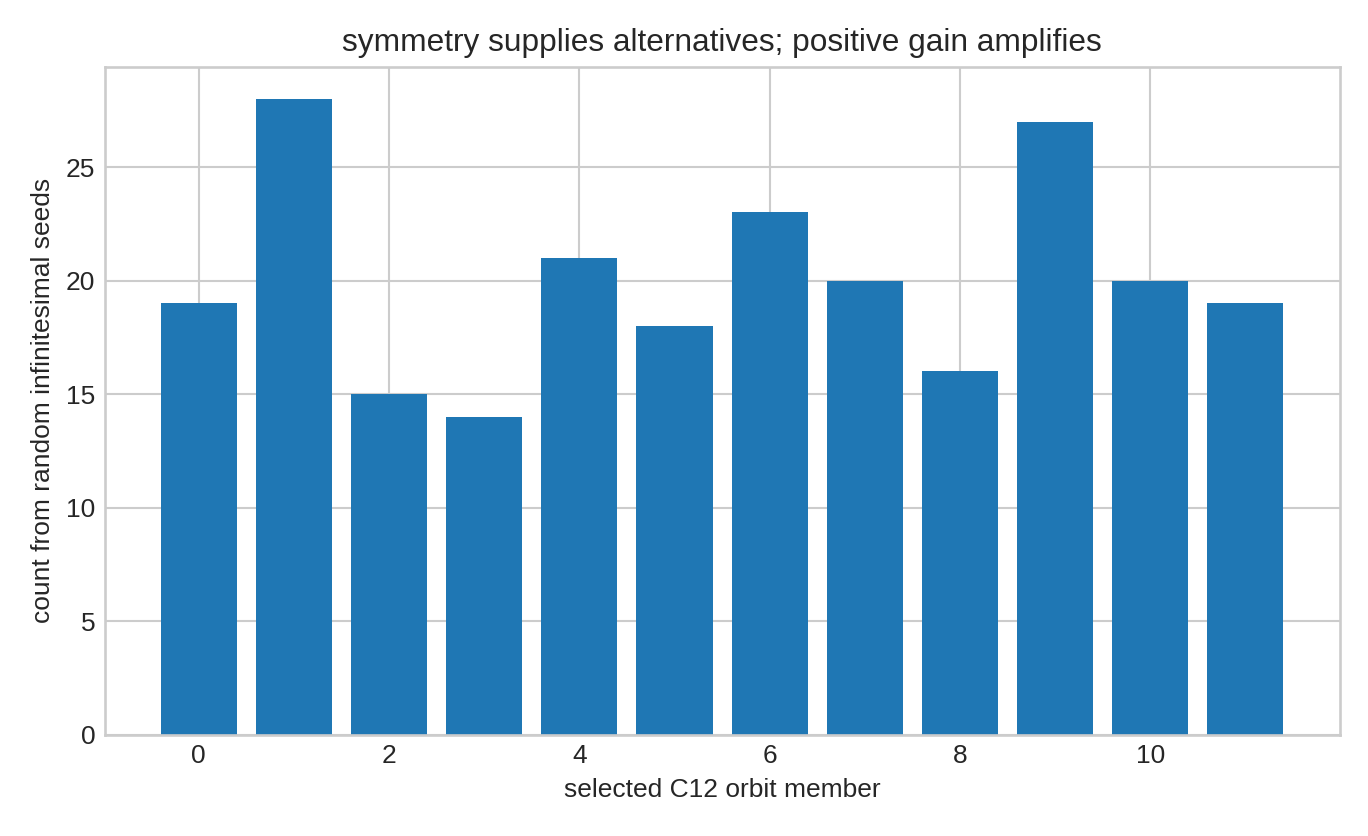
\includegraphics[width=0.74\textwidth]{FIN_ST28_ST45_Figures/st43_symmetry_feedback_selection.png}
\caption{All twelve symmetry-related sectors are realized. Symmetry supplies the alternatives; the positive gain amplifies an initial deviation.}
\end{figure}

ST44 connects this polar mechanism to the actual strict spectrum. The first positive eigenvalue is $0.754121154207$ with a two-dimensional eigenspace. Its projector has uniform diagonal to $3.89\times10^{-16}$, so the subspace is canonical but no axis inside it is. After a conditional axis is selected, the corresponding reflection-symmetric density has orbit size 12, joint commutant dimension 2, and generated algebra dimension 74.

\resultbox{\textbf{Corrected interpretation of ST17.} The strict core is not ``too symmetric'' in a negative sense. It supplies a reservoir of equivalent realizations. What is missing is a strict-sourced instability/gain law and a realized event or record. Symmetry cannot by itself do either job.}

\statusboundary{} The polar-flow coefficients $\mu$, $\varepsilon$, and the saturation are inserted. ST44 demonstrates compatibility with a strict degenerate mode but does not derive positive gain, an individual history, the full algebra, or nontrivial holonomy.

\section{ST45 --- Shared generator is not shared dynamics}

For every positive eigenvalue $\lambda>0$,
\[
|e^{-it\lambda}|=1,
\qquad
|e^{-t\lambda}|<1.
\]
Similarity preserves eigenvalues, so unitary and heat evolution cannot be similar on any positive spectral mode. Their common isomorphic sector is only $\ker A$, which is one-dimensional here. At $t=0.61$, the least-positive heat mode contracts away from one by $0.368725$ while the unitary modulus residual is below $2.0\times10^{-15}$.

The wave channel has yet another functional relation,
\[
C_t=\cos(t\sqrt A),
\]
so its modal frequency scales as $\sqrt\lambda$ rather than $\lambda$. Green poles and Gibbs ratios introduce affine and multiplicative nuisance maps. A common spectral object organizes these channels, but does not erase their dynamical differences.

\begin{theorem}[Representation invariance versus channel inequivalence]
Faithful carrier changes of one complete operational process preserve all records. Unitary, heat, and wave functional calculi of the same $A$ are generally distinct operational processes. A shared generator proves common structure, not identity of information dynamics.
\end{theorem}

\section{Integrated scientific verdict}

\subsection{Does carrier independence have fundamental significance?}

Yes, under a precise restriction. It identifies the candidate fundamental object as an operational equivalence class rather than a material substrate or a coordinate matrix. The invariants are the complete family of operational record probabilities and composition relations. This is stronger than ``the spectrum is information'' and weaker than ``information exists without a carrier.''

For FIN, this is potentially fundamental because it provides a mathematically controlled architecture
\[
\mathfrak I
\xrightarrow{\ \text{faithful representation}\ }
R_i(\mathfrak I).
\]
What remains absent is a theorem that any two real physical media instantiate the same object and a calibration identifying their preparations, instruments, clocks, and records.

\subsection{Can symmetry generate the missing selector?}

Only conditionally. The strict operator provides degenerate modes and hence a space of equivalent choices. A state-dependent observable can enlarge the algebra, and an equivariant positive-gain law can convert an infinitesimal fluctuation into an orbit member. But three sources remain distinct:
\[
\underbrace{\text{symmetry orbit}}_{\text{from }A}
+\underbrace{\text{gain/saturation law}}_{\text{not derived}}
+\underbrace{\text{realized event/record}}_{\text{not supplied}}.
\]
This mechanism therefore gives a disciplined candidate for spontaneous selection, not a discharge of QW-2191.

\subsection{What was falsified?}

\begin{itemize}
\item Spectrum alone is not the carrier-invariant information object.
\item Plain refinement associativity does not select the fine theory.
\item The declared finite-count ST31 protocol does not reliably detect its specified alternative.
\item The constructed ST34 saturation does not produce localization in the performed search.
\item A single state phase cannot produce nontrivial cycle holonomy.
\item One state does not jointly solve canonical selection, full algebra, and gauge flux.
\item Symmetry alone is not positive feedback.
\item A shared $A$ does not make unitary, heat, and wave dynamics equivalent.
\end{itemize}

\subsection{What remains physically missing?}

No program in this release provides a dimensional clock, length or energy calibration; a continuum; a strict-derived nonlinear response or gain law; an apparatus; independently held data; a carrier-to-carrier laboratory equivalence; a legacy-to-strict role-transfer theorem; matter, gauge fields, gravity, or Standard Model dynamics. The results remain local mathematical physics and synthetic receiver analysis.

\section{Recommended programs ST46--ST57}

\begin{longtable}{@{}p{0.07\textwidth}p{0.09\textwidth}p{0.73\textwidth}@{}}
\toprule
ID & Priority & Research program\\
\midrule
\endfirsthead
\toprule
ID & Priority & Research program\\
\midrule
\endhead
ST46 & 1 & Interval-regenerate every strict and memory transcendental coefficient, lifting ST28 from the frozen-decimal model to the complete declared upstream construction.\\
ST47 & 2 & Classify stronger scale-stationary refinement laws capable of coupling or eliminating the free ST30 parameters.\\
ST48 & 3 & Derive or refute positive feedback gain from the strict adaptive law; do not insert $\mu$ silently.\\
ST49 & 4 & Test multi-component or projective state objects for joint selector, full algebra, and $\pi$-holonomy closure.\\
ST50 & 5 & Classify operational intertwiners among unitary, wave, heat, Green, and Gibbs channels, including impossible pairs.\\
ST51 & 6 & Construct finite-count carrier-change tests with two explicitly different encoder/receiver models and frozen record equivalence.\\
ST52 & 7 & Search for an isolated localized saturating-DNLS minimizer orbit and certify its Hessian by interval methods; accept nonexistence if obtained.\\
ST53 & 8 & Add relative entropy, data processing, and entropy-production invariants to the carrier-neutral operational object.\\
ST54 & 9 & Determine whether the ST40 operational equivalence class satisfies a useful categorical universal property rather than only coordinate covariance.\\
ST55 & 10 & Build an executable two-carrier transfer experiment specification without claiming laboratory realization.\\
ST56 & 11 & Audit whether fractal compression can supply a scale-stationary refinement law without hidden selectors or fitted scale parameters.\\
ST57 & 12 & Recompute the minimal axiom graph after ST46--ST56 and test whether one new object pays several currently independent obligations.\\
\bottomrule
\end{longtable}

The highest conceptual payoff is ST48+ST49: they test whether the symmetry reservoir can be converted into an internally generated selector and nontrivial operational structure. The highest proof-completion payoff is ST46. The most direct continuation of the carrier question is ST50+ST51+ST53.

\section{Reproducibility and acceptance tests}

The executable packet contains:
\begin{itemize}
\item \texttt{fin\_st28\_st45\_research.py}: all calculations and figures;
\item \texttt{FIN\_ST28\_ST45\_Results.json}: full result ledger;
\item \texttt{FIN\_ST28\_ST45\_Summary.csv}: compact status table;
\item \texttt{FIN\_ST28\_Jordan\_Root\_Certificate.json}: interval certificate data;
\item two hashed synthetic preregistration packets for ST31 and ST37;
\item \texttt{test\_fin\_st28\_st45.py}: twenty acceptance tests, including live recomputation of the bicommutant and carrier-transport identities.
\end{itemize}

The exact local commands are:
\begin{verbatim}
MPLCONFIGDIR=/tmp/fin-st28-mpl python3 fin_st28_st45_research.py
MPLCONFIGDIR=/tmp/fin-st28-mpl python3 -m unittest -v test_fin_st28_st45.py
\end{verbatim}
The final run returned \texttt{OK} for all twenty tests. Random seeds and software versions are serialized in the results. No external network, laboratory record, or hidden API is required.

\section{Conclusion}

The carrier question does reveal a mathematically fundamental distinction. The object that can survive a change of medium is not a bare message, scalar entropy, or spectrum, but an operational structure transported together with its encoders, dynamics, instruments, composition, and record semantics. This gives FIN a precise research target: derive a carrier-neutral operational object and prove that distinct physical realizations are faithful representations of it.

The symmetry question also yields a sharper architecture. Strict symmetry can provide degenerate possibilities and state orbits. A separate positive-gain instability can amplify a fluctuation, and saturation can stabilize a selected phase. But current FIN derives only the reservoir, not the gain law or realized event. The state can expand the algebra, but one vector still cannot jointly provide canonicity, full algebra, and nontrivial holonomy.

The deepest conclusion surviving the present falsification is therefore:
\[
\boxed{
\begin{minipage}{0.86\textwidth}
FIN currently supplies a finite symmetric spectral organizer from which several inequivalent dynamics can be constructed. Its most coherent informational completion is an operational isomorphism class, while its most coherent selector completion is a state-dependent equivariant bifurcation. Neither completion is yet generated by the strict core or tied to physical carriers, dimensional calibration, and external records.
\end{minipage}}
\]

This is substantial mathematical progress, but not a physical unification theorem and not a Theory-of-Everything closure.

\end{document}
